

\begin{figure}[ht]
\centering
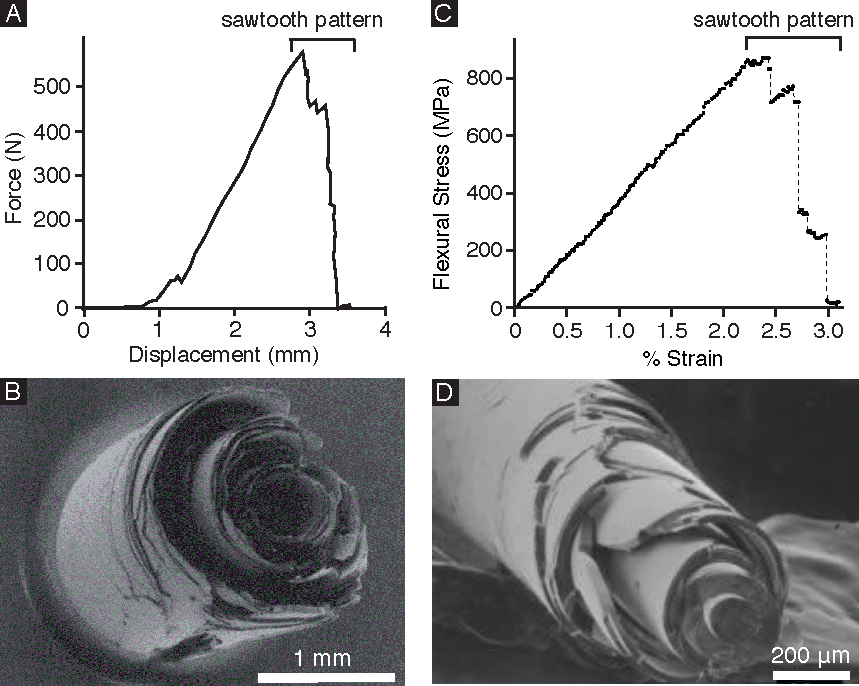
\includegraphics[width=\textwidth]{Figures/Figure2_V7.pdf}
\caption{(\textsf{A}) A force-displacement curve from a three-point bending test performed on a basalia spicule from \textit{Monorhaphis chuni} (\textit{M. chuni})  (adapted from~\cite{levi1989remarkably}). (\textsf{B}) An image of a fractured basalia spicule from \textit{M. chuni} (adapted from~\cite{levi1989remarkably}). (\textsf{C}) A stress-strain curve from a three-point bending test performed on a basalia spicule from \textit{Rosella racovitzea} (\textit{R. racovitzea}) (adapted from~\cite{sarikaya2001biomimetic}). (\textsf{D}) An image of a fractured basalia spicule from \textit{R. racovitzea} tested in three-point bending (modified from~\cite{sarikaya2001biomimetic}). }
\label{fig:sawtoothlit}
\end{figure}
